\documentclass[a4paper,14pt]{article}

%%% Работа с русским языком
\usepackage{cmap}					% поиск в PDF
\usepackage{mathtext} 				% русские буквы в формулах
\usepackage[T2A]{fontenc}			% кодировка
\usepackage[utf8]{inputenc}			% кодировка исходного текста
\usepackage[english,russian]{babel}	% локализация и переносы
\usepackage{indentfirst}
\frenchspacing

\newcommand{\vyp}{\ensuremath{\hookrightarrow}}
\renewcommand{\epsilon}{\ensuremath{\varepsilon}}
\renewcommand{\phi}{\ensuremath{\varphi}}
\renewcommand{\kappa}{\ensuremath{\varkappa}}
\renewcommand{\le}{\ensuremath{\leqslant}}
\renewcommand{\leq}{\ensuremath{\leqslant}}
\renewcommand{\ge}{\ensuremath{\geqslant}}
\renewcommand{\geq}{\ensuremath{\geqslant}}
\renewcommand{\emptyset}{\varnothing}
\newcommand{\Ra}{\ensuremath{\Rightarrow}}
\newcommand{\ra}{\ensuremath{\rightarrow}}
\newcommand{\LRa}{\ensuremath{\Leftrightarrow}}
\newcommand{\tbf}{\textbf}
\newcommand{\ov}{\ensuremath{\overline}}
\newcommand{\CC}{\ensuremath{\mathbb{C}}}
\newcommand{\RR}{\ensuremath{\mathbb{R}}}
\newcommand{\NN}{\ensuremath{\mathbb{N}}}
\newcommand{\QQ}{\ensuremath{\mathbb{Q}}}
\newcommand{\ZZ}{\ensuremath{\mathbb{Z}}}

%%% Дополнительная работа с математикой
\usepackage{amsmath,amsfonts,amssymb,amsthm,mathtools} % AMS
\usepackage{icomma} % "Умная" запятая: $0,2$ --- число, $0, 2$ --- перечисление

%% Номера формул
%\mathtoolsset{showonlyrefs=true} % Показывать номера только у тех формул, на которые есть \eqref{} в тексте.
%\usepackage{leqno} % Нумереация формул слева

%% Свои команды
\DeclareMathOperator{\sgn}{\mathop{sgn}}

%% Перенос знаков в формулах (по Львовскому)
\newcommand*{\hm}[1]{#1\nobreak\discretionary{}
{\hbox{$\mathsurround=0pt #1$}}{}}



%%% Работа с картинками
\usepackage{graphicx}  % Для вставки рисунков
\graphicspath{{images/}{images2/}}  % папки с картинками
\setlength\fboxsep{3pt} % Отступ рамки \fbox{} от рисунка
\setlength\fboxrule{1pt} % Толщина линий рамки \fbox{}
\usepackage{wrapfig} % Обтекание рисунков текстом

%%% Работа с таблицами
\usepackage{array,tabularx,tabulary,booktabs} % Дополнительная работа с таблицами
\usepackage{longtable}  % Длинные таблицы
\usepackage{multirow} % Слияние строк в таблице

%%% Теоремы
\theoremstyle{plain} % Это стиль по умолчанию, его можно не переопределять.
\newtheorem{theorem}{Теорема}[section]
\newtheorem{proposition}[theorem]{Утверждение}
 
\theoremstyle{definition} % "Определение"
\newtheorem{corollary}{Следствие}[theorem]
\newtheorem{problem}{Задача}[section]
 
\theoremstyle{remark} % "Примечание"
\newtheorem*{nonum}{Решение}

%%% Программирование
\usepackage{etoolbox} % логические операторы

%%% Страница
\usepackage{extsizes} % Возможность сделать 14-й шрифт
\usepackage{geometry} % Простой способ задавать поля
	\geometry{top=20mm}
	\geometry{bottom=20mm}
	\geometry{left=5mm}
	\geometry{right=15mm}
 %
\usepackage{fancyhdr} % Колонтитулы
 	\pagestyle{fancy}
 	\renewcommand{\headrulewidth}{1pt}  % Толщина линейки, отчеркивающей верхний колонтитул
%\fancypagestyle{firstpage}{
	\rhead{\large{Исыпов Илья}}
%}
% 	\lfoot{Нижний левый}
% 	\rfoot{\large{Рябых Владислав, Б05-905}}
% 	\rhead{Верхний правый]}
% 	\chead{Верхний в центре}
 	\lhead{\large{Рябых Владислав}}
%	\cfoot{Нижний в центре} % По умолчанию здесь номер страницы

\usepackage{setspace} % Интерлиньяж
\onehalfspacing % Интерлиньяж 1.5
%\doublespacing % Интерлиньяж 2
%\singlespacing % Интерлиньяж 1

\usepackage{lastpage} % Узнать, сколько всего страниц в документе.

\usepackage{soul} % Модификаторы начертания

\usepackage{hyperref}
\usepackage[usenames,dvipsnames,svgnames,table,rgb]{xcolor}
\hypersetup{				% Гиперссылки
    unicode=true,           % русские буквы в раздела PDF
    pdftitle={Заголовок},   % Заголовок
    pdfauthor={Автор},      % Автор
    pdfsubject={Тема},      % Тема
    pdfcreator={Создатель}, % Создатель
    pdfproducer={Производитель}, % Производитель
    pdfkeywords={keyword1} {key2} {key3}, % Ключевые слова
    colorlinks=true,       	% false: ссылки в рамках; true: цветные ссылки
    linkcolor=red,          % внутренние ссылки
    citecolor=black,        % на библиографию
    filecolor=magenta,      % на файлы
    urlcolor=cyan           % на URL
}

\usepackage{csquotes} % Еще инструменты для ссылок

%\usepackage[style=authoryear,maxcitenames=2,backend=biber,sorting=nty]{biblatex}

\usepackage{multicol} % Несколько колонок

\usepackage{tikz} % Работа с графикой
\usepackage{pgfplots}
\usepackage{pgfplotstable}

\usepackage{caption}
\long\def\comment{}
\setlength{\abovecaptionskip}{7pt}
\setlength{\belowcaptionskip}{7pt}


\begin{document}
\author{Рябых Владислав и Исыпов Илья, Б05-905}
\title{\tbf{3.2.2. Резонанс напряжений}}
\maketitle

\tbf{Цель работы:} исследование резонанса напряжений в последовательном колебательном контуре с изменяемой ёмкостью, включающее получение амплитудно-частотных и фазово-частотных характеристик, а также определение основных параметров контура.

\tbf{В работе используются:} генератор сигналов, источник напряжения, нагруженный на последовательный колебательный контур с переменной ёмкостью, двулучевой осциллограф, цифровые вольтметры.


\section*{Экспериментальная установка}

\begin{center}
	\begin{figure}[bhtp]
		\centering
		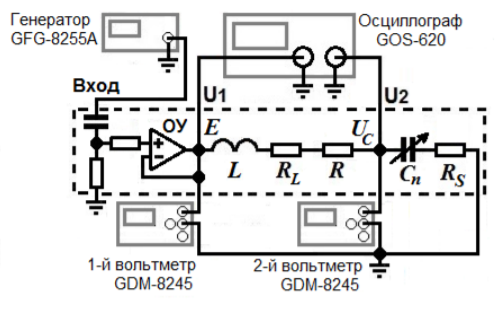
\includegraphics[width=0.7\linewidth]{scheme.png}
		\caption{Схема установки для исследования свободных колебаний}
		\label{scheme}
	\end{figure}
\end{center}


Схема экспериментального стенда для изучения резонанса напряжений в последовательном колебательном контуре показана на рис. \ref{scheme}. Синусоидальный сигнал от генератора GFG8255A поступает через согласующую RC-цепочку на вход источника напряжения, собранного на операционном усилителе ОУ. Питание операционного усилителя осуществляется
встроенным блоком-выпрямителем от сети переменного тока 220 Вольт (цепь питания на
схеме не показана). Источник напряжения, обладающий по определению нулевым внутренним сопротивлением, фактически обеспечивает с высокой точностью постоянство амплитуды сигнала на меняющейся по величине нагрузке – последовательном колебательном контуре, изображенном на рисунке в виде эквивалентной схемы.


\section*{Ход работы}

\begin{enumerate}


\item Подготавливаем установку к работе и включаем приборы.

\item Выставляем на входе контура напряжение $E = 175.5~\text{мВ}$, в течение всей работы поддерживая его постоянным.

\item Добиваемся получения двух отцентрированных синусоид на осциллографе. Убеждаемся, что одна из синусоид при изменении частоты $f$ генератора меняет амплитуду относительно начала координат, в то время как амплитуда другой не меняется с погрешностью не более 1\%.

\item Для контуров с семью различными ёмкостями, меняя их с помощью переключателя на
блоке, измеряем резонансные частоты $f_{0n}$ и напряжения $U_C(f_{0n})$. Регистрируем также
напряжения $E(f_{0n})$, игнорируя отклонения в пределах относительной погрешности 1\%.

\item Для контуров ёмкостями $C_2 = 47.6~\text{нФ}$ и $C_5 = 68.0~\text{нФ}$ снимаем амплитудно-частотные характеристики $U(f)$ при том же напряжении $E$.

\begin{table}[hbt!]
\begin{center}
	\begin{tabular}{ccccc||c|c|c|c|c|}
		\hline
		\multicolumn{5}{|c||}{$C_2 = 47.6$ нФ}                                                                                                         & \multicolumn{5}{c|}{$C_5 = 68.0$ нФ}        \\ \hline
		\multicolumn{1}{|c|}{$n$} & \multicolumn{1}{c|}{$f$, кГц} & \multicolumn{1}{c|}{$\sigma_f$, кГц} & \multicolumn{1}{c|}{$A$, В} & $\sigma_A$, В         & $n$ & f, кГц & $\sigma_f$, кГц & A, В & $\sigma_A$, В \\ \hline
		\multicolumn{1}{|c|}{1}   & \multicolumn{1}{c|}{23.27}     & \multicolumn{1}{c|}{0.1}             & \multicolumn{1}{c|}{3.30}   & 0.01                  & 1   & 19.60     & 0.1             & 2.89 & 0.01          \\ \hline
		\multicolumn{1}{|c|}{2}   & \multicolumn{1}{c|}{23.49}     & \multicolumn{1}{c|}{0.1}             & \multicolumn{1}{c|}{3.10}   & 0.01                  & 2   & 19.32   & 0.1             & 2.54 & 0.01          \\ \hline
		\multicolumn{1}{|c|}{3}   & \multicolumn{1}{c|}{23.66}       & \multicolumn{1}{c|}{0.1}             & \multicolumn{1}{c|}{2.80}   & 0.01                  & 3   & 19.20   & 0.1             & 2.28 & 0.01          \\ \hline
		\multicolumn{1}{|c|}{4}   & \multicolumn{1}{c|}{23.84}     & \multicolumn{1}{c|}{0.1}             & \multicolumn{1}{c|}{2.49}   & 0.01                  & 4   & 19.00   & 0.1             & 1.93 & 0.01          \\ \hline
		\multicolumn{1}{|c|}{5}   & \multicolumn{1}{c|}{24.03}       & \multicolumn{1}{c|}{0.1}             & \multicolumn{1}{c|}{2.15}   & 0.01                  & 5   & 18.94     & 0.1             & 1.81 & 0.01          \\ \hline
		\multicolumn{1}{|c|}{6}   & \multicolumn{1}{c|}{24.15}     & \multicolumn{1}{c|}{0.1}             & \multicolumn{1}{c|}{1.96}   & 0.01                  & 6   & 18.77   & 0.1             & 1.57 & 0.01          \\ \hline
		\multicolumn{1}{|c|}{7}   & \multicolumn{1}{c|}{24.49}     & \multicolumn{1}{c|}{0.1}             & \multicolumn{1}{c|}{1.55}   & 0.01                  & 7   & 18.55   & 0.1             & 1.34 & 0.01          \\ \hline
		\multicolumn{1}{|c|}{8}   & \multicolumn{1}{c|}{25.12}     & \multicolumn{1}{c|}{0.1}             & \multicolumn{1}{c|}{1.07}   & 0.01                  & 8   & 18.19   & 0.1             & 1.06 & 0.01          \\ \hline
		\multicolumn{1}{|c|}{9}   & \multicolumn{1}{c|}{23.21}     & \multicolumn{1}{c|}{0.1}             & \multicolumn{1}{c|}{3.34}   & 0.01                  & 9   & 19.55     & 0.1             & 2.86  & 0.01          \\ \hline
		\multicolumn{1}{|c|}{10}  & \multicolumn{1}{c|}{23.00}     & \multicolumn{1}{c|}{0.1}             & \multicolumn{1}{c|}{3.05}   & 0.01                  & 10  & 19.88   & 0.1             & 2.66 & 0.01          \\ \hline
		\multicolumn{1}{|c|}{11}  & \multicolumn{1}{c|}{22.90}     & \multicolumn{1}{c|}{0.1}             & \multicolumn{1}{c|}{2.83}   & 0.01                  & 11  & 20.00   & 0.1             & 2.47 & 0.01          \\ \hline
		\multicolumn{1}{|c|}{12}  & \multicolumn{1}{c|}{22.74}     & \multicolumn{1}{c|}{0.1}             & \multicolumn{1}{c|}{2.47}   & 0.01                  & 12  & 20.18   & 0.1             & 2.17  & 0.01          \\ \hline
		\multicolumn{1}{|c|}{13}  & \multicolumn{1}{c|}{22.49}       & \multicolumn{1}{c|}{0.1}             & \multicolumn{1}{c|}{1.97}   & 0.01                  & 13  & 20.27   & 0.1             & 2.01 & 0.01          \\ \hline
		\multicolumn{1}{|c|}{14}  & \multicolumn{1}{c|}{22.32}     & \multicolumn{1}{c|}{0.1}             & \multicolumn{1}{c|}{1.72}   & 0.01                  & 14  & 20.41   & 0.1             & 1.80 & 0.01          \\ \hline
		\multicolumn{1}{|c|}{15}  & \multicolumn{1}{c|}{21.99}     & \multicolumn{1}{c|}{0.1}             & \multicolumn{1}{c|}{1.37}   & 0.01                  & 15  & 20.72   & 0.1             & 1.43 & 0.01          \\ \hline
		\multicolumn{1}{|c|}{16}  & \multicolumn{1}{c|}{21.45}     & \multicolumn{1}{c|}{0.1}             & \multicolumn{1}{c|}{1.02}   & 0.01                  & 16  & 21.20   & 0.1             & 1.05 & 0.01          \\ \hline
	\end{tabular}
\end{center}
\caption{Результаты измерений}
\end{table}


\item По данным из таблицы 1 построим на одном графике амплитудо-частотные характеристики в координатах $f, U$. См. рис. \ref{gr1}


\begin{center}
	\begin{figure}[bhtp]
		\centering
		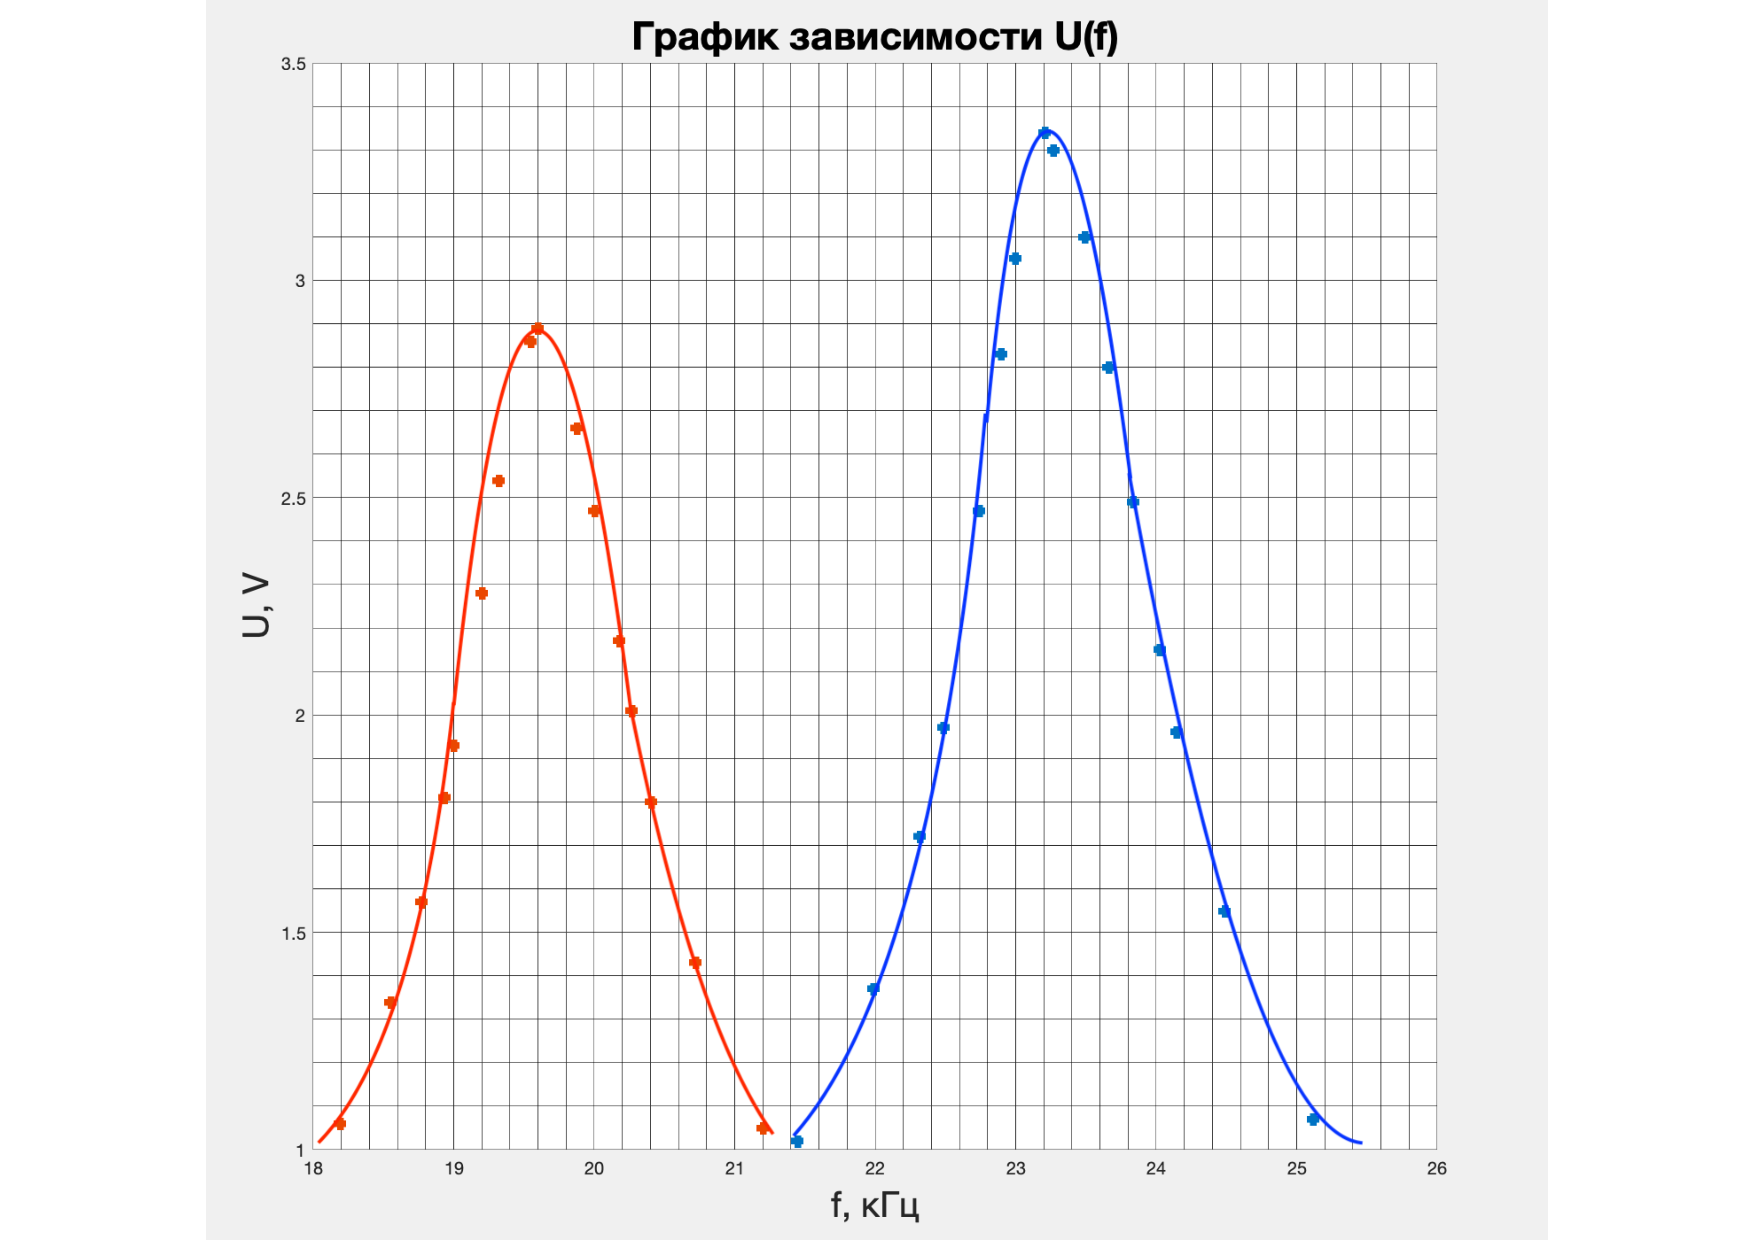
\includegraphics[width=0.77\linewidth]{gr1.pdf}
		\caption{Амплитудно-частотные характеристики}
		\label{gr1}
	\end{figure}
\end{center}


\item По тем же данным таблицы 1 построим на одном графике амплитудо-частотные характеристики в безразмерных координатах $f/f_0, U/U_0$. См. рис. \ref{gr2}. По ширине резонансных кривых на уровне определим добротности $Q$ соответствующих контуров: $Q_{C_2} = 20.6$ и $Q_{C_5} = 17.2$.

\begin{center}
	\begin{figure}[bhtp]
		\centering
		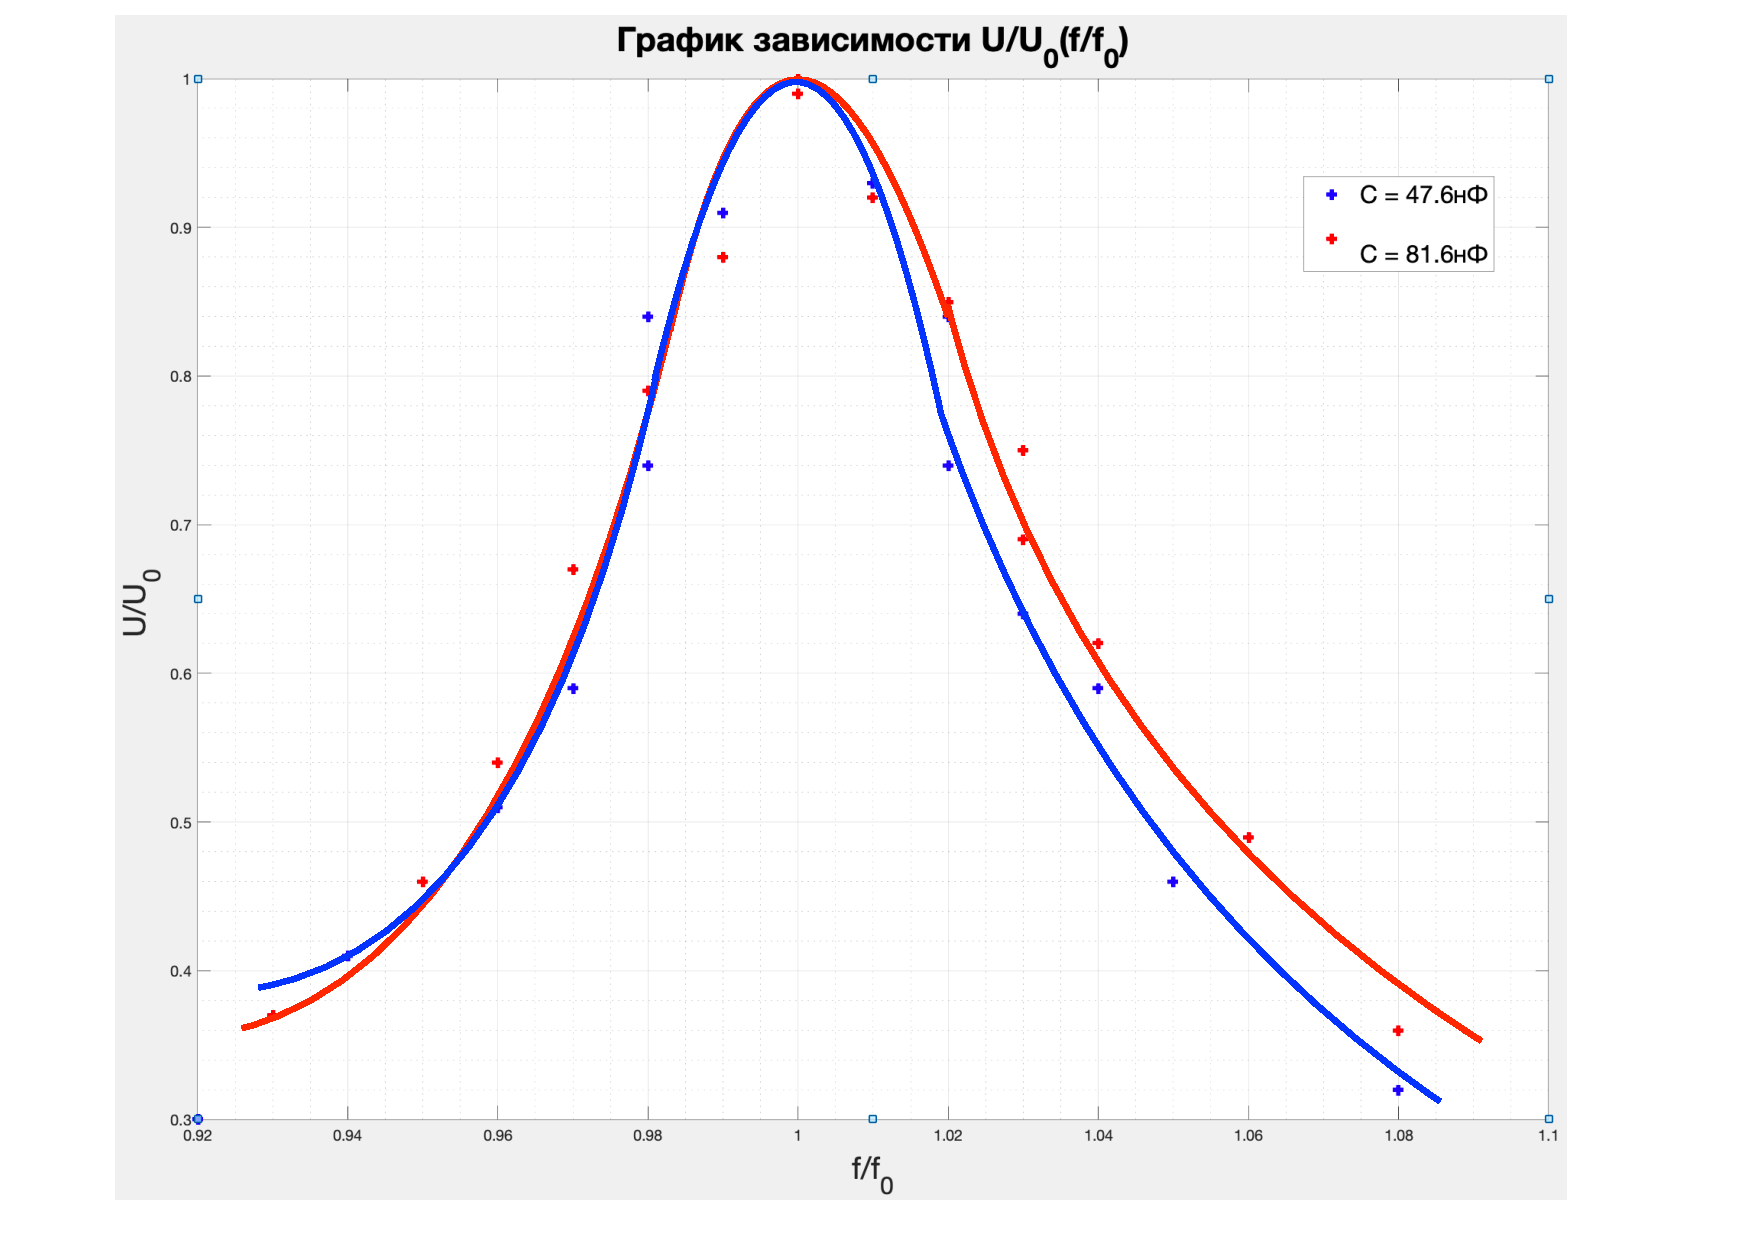
\includegraphics[width=0.75\linewidth]{l322_l2.pdf}
		\caption{Амплитудно-частотные характеристики}
		\label{gr2}
	\end{figure}
\end{center}


\newpage

\item Для тех же двух контуров снимаем фазово-частотные характеристики $\phi_C(f)$ при том же напряжении $E$.


\begin{table}[hbt!]
\begin{center}
	\begin{tabular}{ccc||c|c|c|}
		\hline
		\multicolumn{3}{|c||}{$C_2 = 47.6 $ нФ} & \multicolumn{3}{c|}{$C_5 = 68.0$ нФ} \\ \hline
		\multicolumn{1}{|c|}{$n$} & \multicolumn{1}{c|}{$f$, кГц} & $-\phi/ \pi$ & $n$ & $f$, кГц & $-\phi/ \pi$ \\ \hline
		\multicolumn{1}{|c|}{1} & \multicolumn{1}{c|}{23.21} & 0.46 & 1 & 19.65 & 0.48 \\ \hline
		\multicolumn{1}{|c|}{2} & \multicolumn{1}{c|}{23.47} & 0.61 & 2 & 19.27 & 0.32 \\ \hline
		\multicolumn{1}{|c|}{3} & \multicolumn{1}{c|}{23.57} & 0.64 & 3 & 19.13 & 0.24 \\ \hline
		\multicolumn{1}{|c|}{4} & \multicolumn{1}{c|}{23.69} & 0.69 & 4 & 18.91 & 0.20 \\ \hline
		\multicolumn{1}{|c|}{5} & \multicolumn{1}{c|}{23.93} & 0.75 & 5 & 18.76 & 0.18 \\ \hline
		\multicolumn{1}{|c|}{6} & \multicolumn{1}{c|}{24.26} & 0.80 & 6 & 18.56 & 0.13 \\ \hline
		\multicolumn{1}{|c|}{7} & \multicolumn{1}{c|}{24.56} & 0.83 & 7 & 18.27 & 0.11 \\ \hline
		\multicolumn{1}{|c|}{8} & \multicolumn{1}{c|}{25.11} & 0.88 & 8 & 18.03 & 0.09 \\ \hline
		\multicolumn{1}{|c|}{9} & \multicolumn{1}{c|}{23.20} & 0.46 & 9 & 19.61 & 0.49 \\ \hline
		\multicolumn{1}{|c|}{10} & \multicolumn{1}{c|}{22.95} & 0.34 & 10 & 19.86 & 0.60 \\ \hline
		\multicolumn{1}{|c|}{11} & \multicolumn{1}{c|}{22.77} & 0.27 & 11 & 19.98 & 0.65 \\ \hline
		\multicolumn{1}{|c|}{12} & \multicolumn{1}{c|}{22.67} & 0.23 & 12 & 20.24 & 0.74 \\ \hline
		\multicolumn{1}{|c|}{13} & \multicolumn{1}{c|}{22.51} & 0.18 & 13 & 20.43 & 0.76 \\ \hline
		\multicolumn{1}{|c|}{14} & \multicolumn{1}{c|}{22.20} & 0.14 & 14 & 20.68 & 0.82 \\ \hline
		\multicolumn{1}{|c|}{15} & \multicolumn{1}{c|}{21.71} & 0.10 & 15 & 20.84 & 0.83 \\ \hline
		\multicolumn{1}{|c|}{16} & \multicolumn{1}{c|}{21.35} & 0.08 & 16 & 21.15 & 0.86 \\ \hline
	\end{tabular}
\end{center}
\caption{Результаты измерений}
\end{table}

\item По данным таблицы 2 построим на одном графике фазово-частотные характеристики в координатах $f/f_0,\phi_C /\pi$ для выбранных контуров. См. рис. \ref{gr3}. По этим характеристикам определим добротности контуров: $Q_{C_2} = 20$ и $Q_{C_5} = 16.4$.

\begin{center}
	\begin{figure}[bhtp]
		\centering
		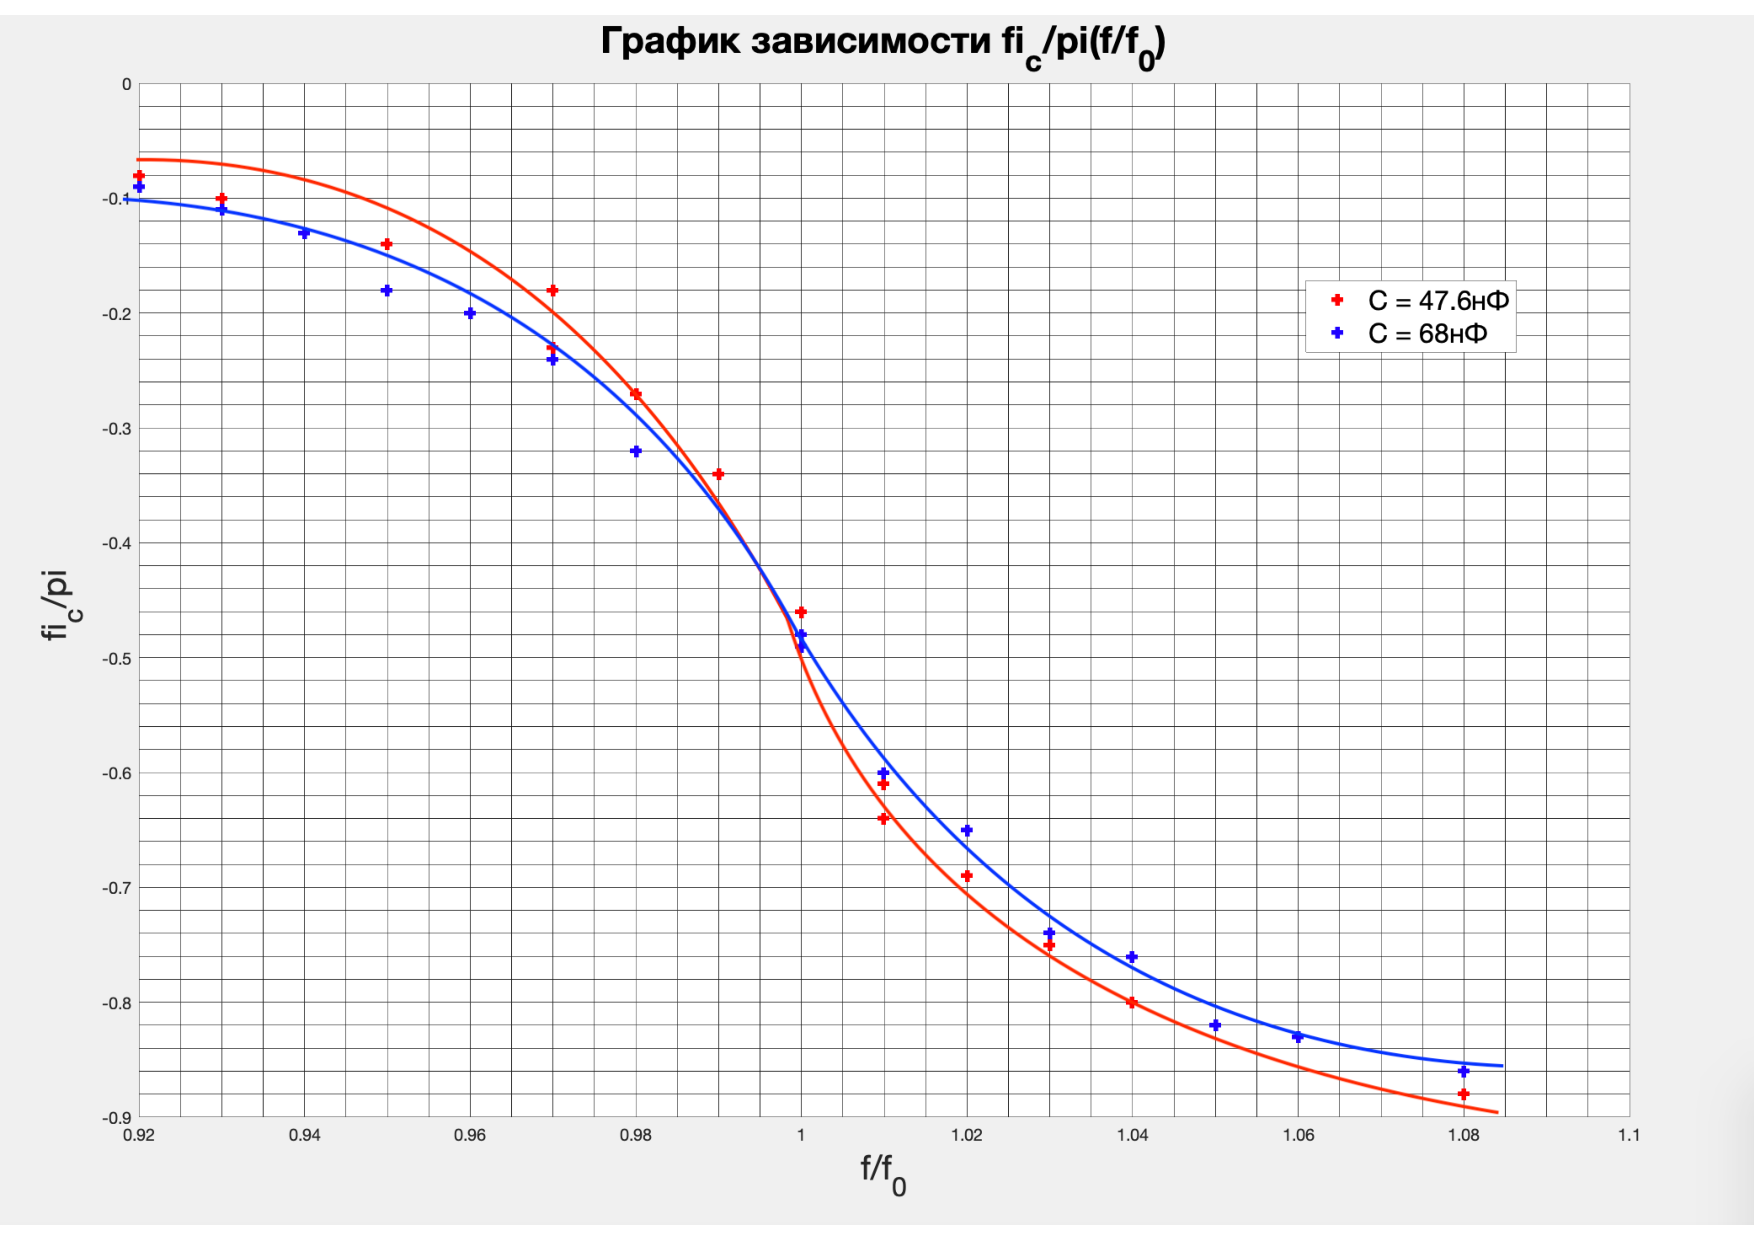
\includegraphics[width=\linewidth]{gr3.pdf}
		\caption{Фазово-частотные характеристики}
		\label{gr3}
	\end{figure}
\end{center}


\clearpage


\item Результаты измерений представим в таблице.


\begin{table}[hbt!]
	\centering
	\begin{tabular}{|c|c|c|c|c|c|c|c|c|c|c|c|}
		\hline
		$n$ & $C_n$, нФ & \begin{tabular}[c]{@{}c@{}}$f_{0n}$, \\ кГц\end{tabular} & $U_C$, В & $E$, мВ & \begin{tabular}[c]{@{}c@{}}$L$, \\ мкГн\end{tabular} & $Q$ & \begin{tabular}[c]{@{}c@{}}$\rho$, \\ Ом\end{tabular} & \begin{tabular}[c]{@{}c@{}}$R_{\sum}$, \\ Ом\end{tabular} & \begin{tabular}[c]{@{}c@{}}$R_{S_{\max}}$,\\ Ом\end{tabular} & $R_L$, Ом & $I$, мА \\ \hline
		1 & 24.8 & 32.20 & 4.38 & 175.5 & 986.1 & 25.0 & 199.4 & 7.99 & 0.20 & 4.34 & 21.97 \\ \hline
		2 & 33.2 & 27.78 & 3.88 & 175.5 & 989.6 & 22.1 & 172.7 & 7.81 & 0.17 & 4.19 & 22.47 \\ \hline
		3 & 47.6 & 23.27 & 3.35 & 175.5 & 983.7 & 19.1 & 143.8 & 7.53 & 0.14 & 3.94 & 23.30 \\ \hline
		4 & 57.5 & 21.17 & 3.10 & 175.5 & 983.9 & 17.7 & 130.8 & 7.41 & 0.13 & 3.82 & 23.70 \\ \hline
		5 & 68.0 & 19.42 & 2.88 & 175.5 & 988.7 & 16.4 & 120.6 & 7.35 & 0.12 & 3.78 & 23.88 \\ \hline
		6 & 81.6 & 17.73 & 2.90 & 175.5 & 988.5 & 16.5 & 110.1 & 6.66 & 0.11 & 3.63 & 26.35 \\ \hline
		7 & 102.8 & 15.82 & 2.42& 175.5 & 985.5 & 13.8 & 97.9  & 7.10 & 0.10 & 3.55 & 24.72 \\ \hline
		\multicolumn{5}{|c|}{Среднее значение} & 986.6 & 18.6 & 139.3 & 7.41 & 0.14 & 3.89 & 23.77 \\ \hline
		\multicolumn{5}{|c|}{Коэффициент Стьюдента} & 2.23 & \multicolumn{4}{c|}{--} & 2.26 & -- \\ \hline
	\end{tabular}
\end{table}


\item По данным таблицы построим график зависимости $R_L(f_0)$, также нанесём на него прямую $\langle R_L \rangle$. См. рис. \ref{gr4}

\begin{center}
	\begin{figure}[bhtp!]
		\centering
		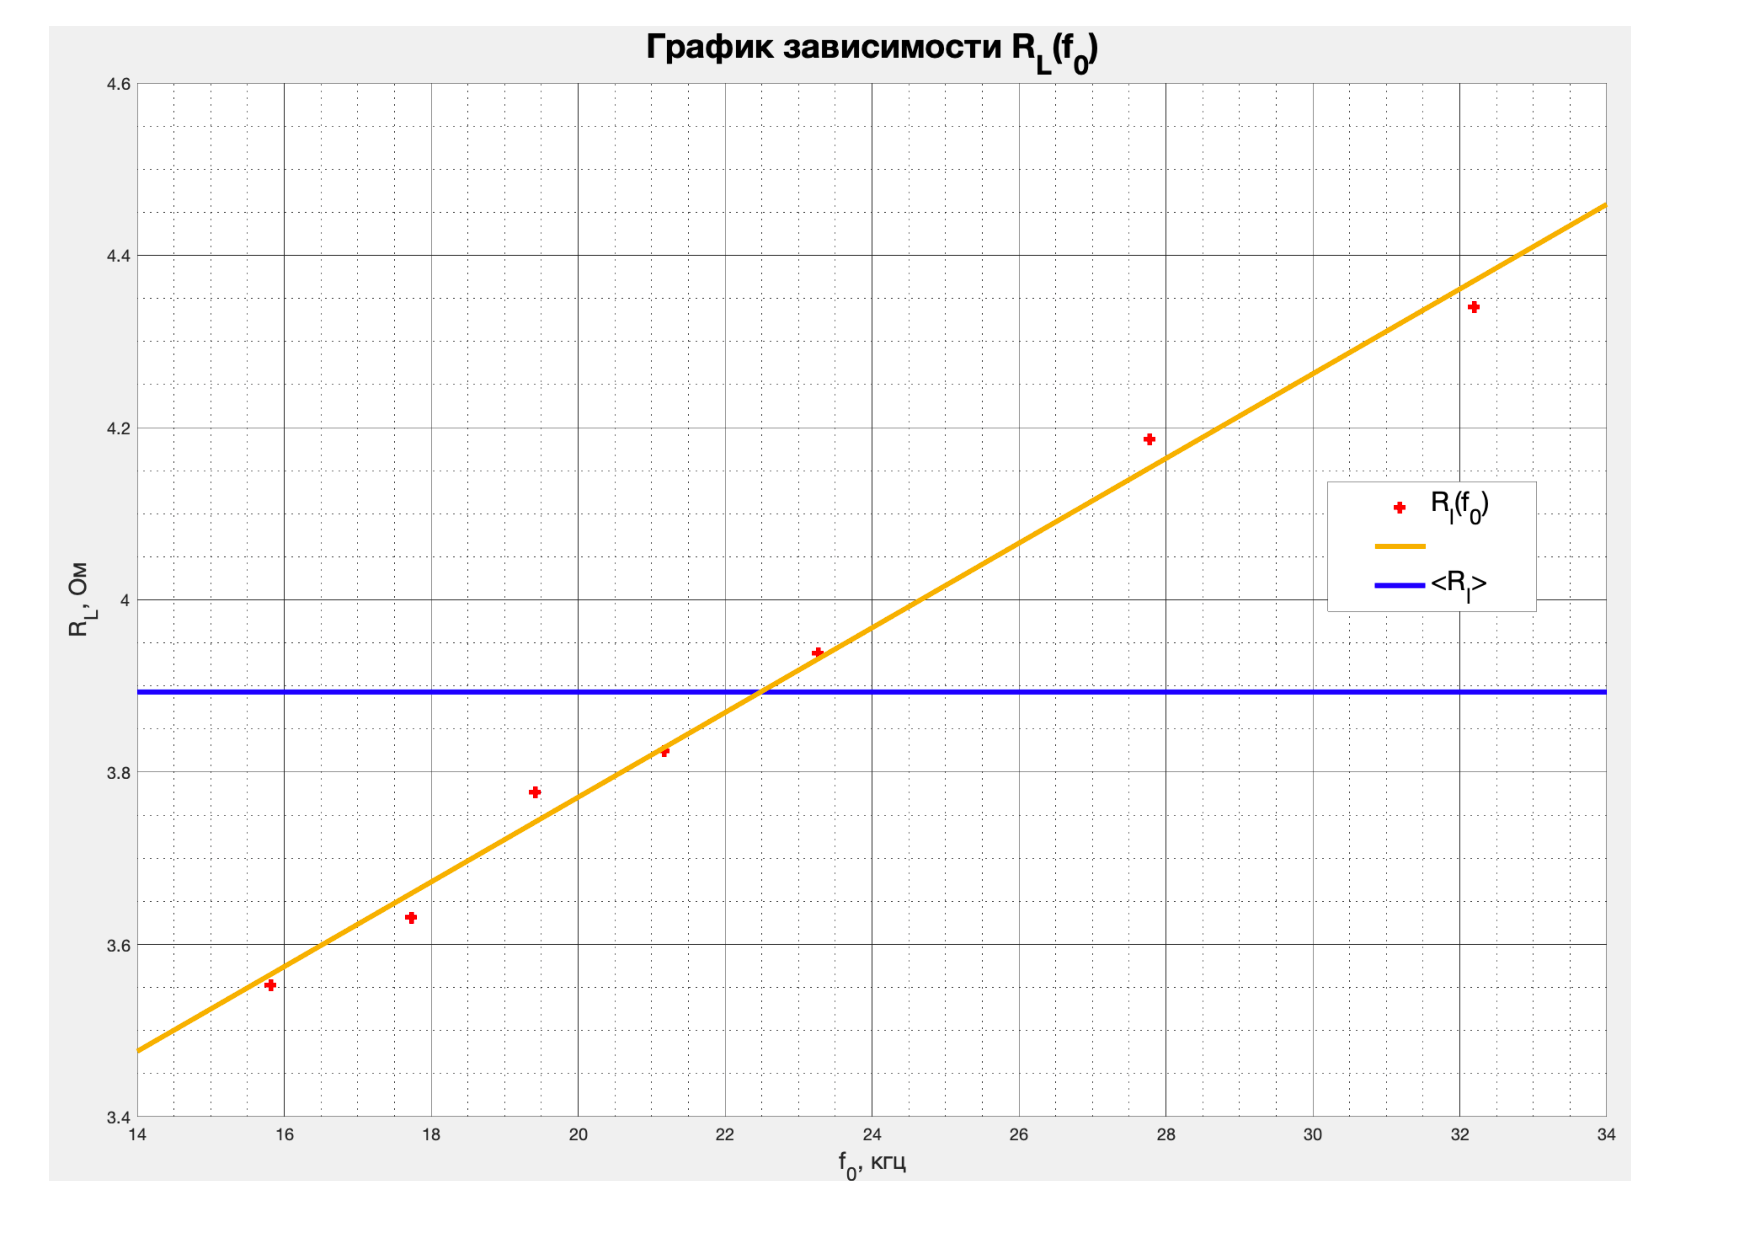
\includegraphics[width=0.75\linewidth]{gr4.pdf}
		\caption{график зависимости $R_L(f_0)$}
		\label{gr4}
	\end{figure}
\end{center}


\end{enumerate}

\section*{Выводы}

В данной работе мы исследовали резонансы напряжений в последовательном колебательном контуре с изменяемой ёмкостью, получали амплитудно-частотные характеристики, а также определили основные параметры контура.


\end{document}